\subsubsection{Reconstruction Overview}

The angiograms is a procedure of projecting 3D objects to 2D
projection space during which many details may disappear and
foreshorten as well as overlapping. Just using the 2D projections to
justify the patient's conditions has inherent limitations. Using two
or several projections from multi views to reconstruct the topological
structures of the coronary arteries in 3D space is a useful method
during heart operations such as intervening.

The reconstruction of the coronary arteries are regarded to the type
of the X-Ray machines which can be divided into single-plane and
biplane machines. The reconstruction based on single-plane angiospasm
is to obtain several angles of views at the same moment of different
cardiac cycles, and uses these projections to reconstruct the vessels.
The difference between the biplane and the single-plane
reconstructions is biplane systems can achieve two synchronous
projection pairs at the same time without time error, leading to less
deformation of the vessels and high accuracy. For the reason that
biplane systems are much more expensive than single-planes and not common
in ordinary hospitals, we focus on the reconstruction of single-plane systems.

In order to reconstruct the 3D vessels, it is important to find the
corresponding points on each angiograms of different views for all 3D
points. In typical methods registration of the images between
different projection views are needed. However, there are problems
they are facing. No matter registrations based on features such as
bifurcations or any others, the first problem they are facing is that
the registration results are mostly not good enough even with many mistakes if
the changes among the views are large. The mistakes during
registration may lead to much more huge errors during the
reconstruction. The second problem is that these kinds of methods are
so fixed that neither constraints such as the connectivity of the
vessel neighbours nor some known conditions or knowledge can be added
which lead to a great waste of the various original information.

\subsubsection{Our Method}
The imaging modality of the X-Ray angiograms is different from the
ways other imaging devices such as cameras or vidicons work in. The
light source is the X-Ray source and the imaging plane is the
intensifier. The imaging procedure is mostly like perspective
projection under 3D space. We simulated this procedure using OpenGL.
This can be described in Figure \ref{fig:xray_work_way}

\begin{figure}
 \centering
  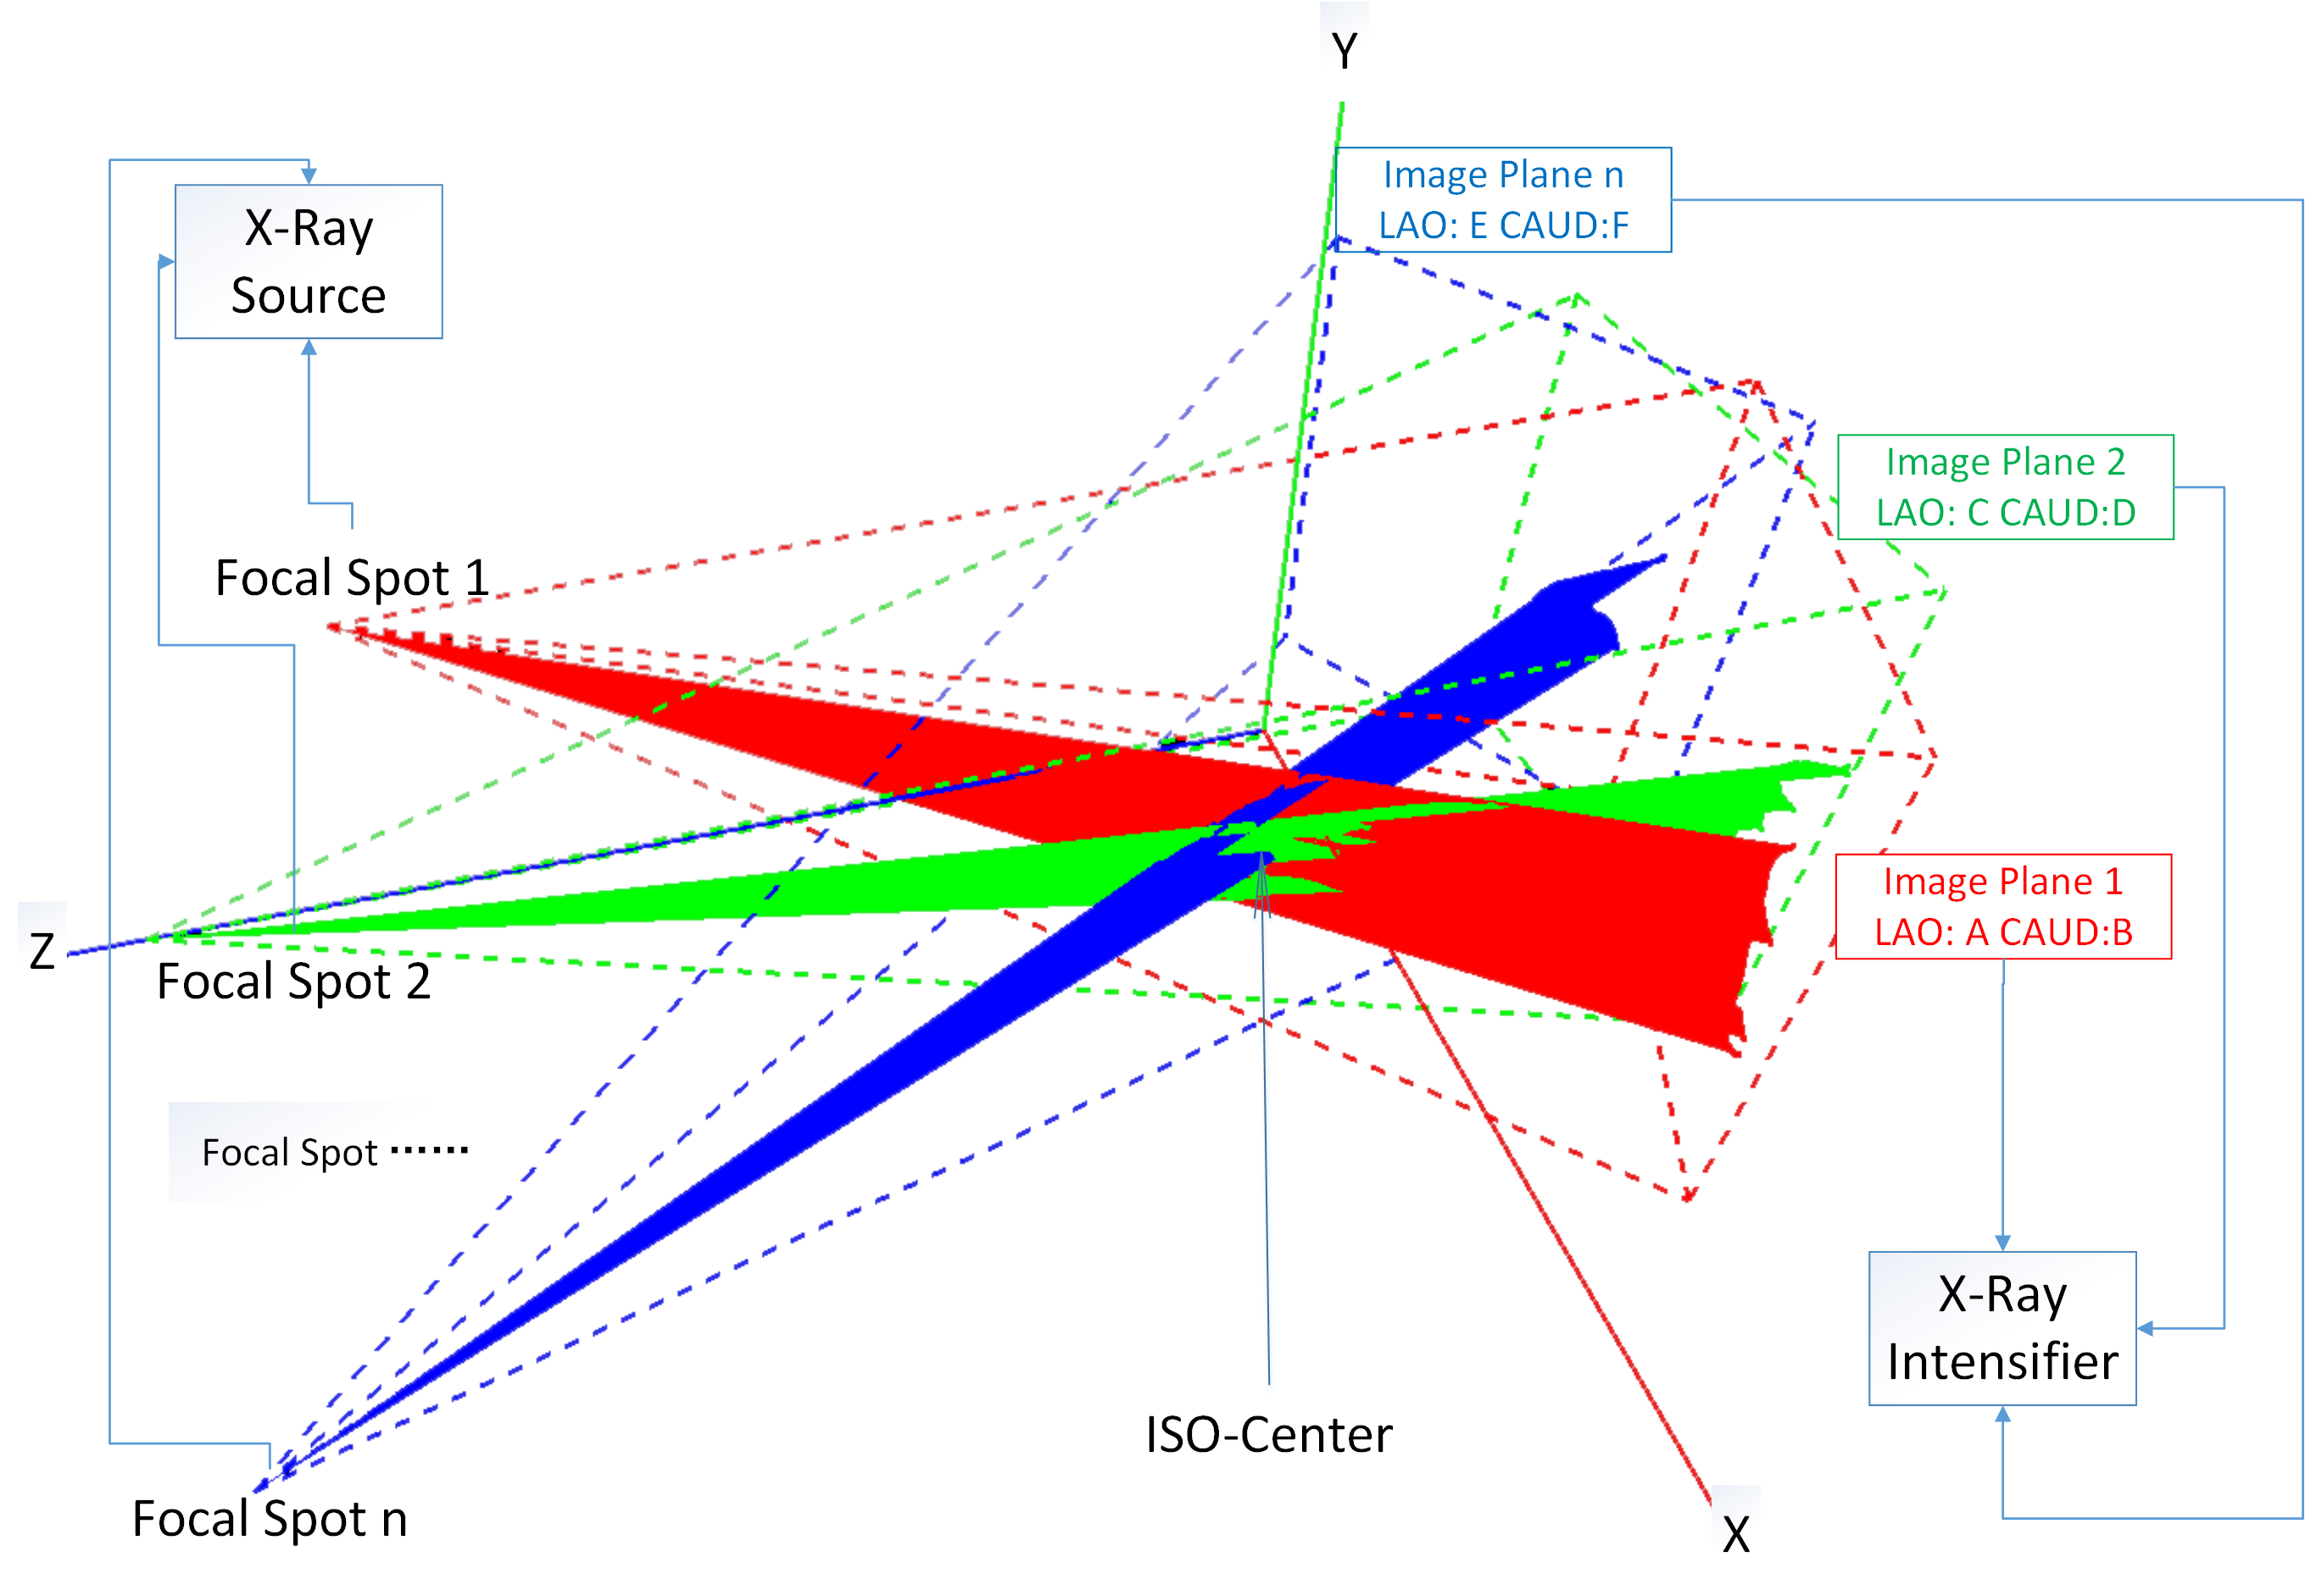
\includegraphics[width=3.0in]{x_ray_work.png}\\
  \caption{X-Ray Perspective Projection Of Vessel Skeletons}\label{fig:xray_work_way}
\end{figure}

The frustum of each color represents one view of the angiograms. The
source of the frustum could be seen as X-Ray source, while the far
plane could be seen as the intensifier. The vessel skeletons should be
at the iso-center. The exact intersected lines from every view should
be 3D space structures of the skeletons of the projected vessels.
Being aware of the diameters at every skeleton point, we can get the
structures of the vessels.

But the intersections are the correspondence between view pairs. The
computation of intersection lines (points) goes back to the
registration problem which are ill-posed. Also, due to precision and
other errors, it is hard to obtain the accurate intersections among
all the views.

However, on the other hand, the 3D skeletons could be regarded as
consisting of several skeleton segments. Each segment could be seen as
made up of sampled points. These points must be between the space of
the X-Ray source and the intensifier. Also, they should be mostly
projected onto every view.  So, if we sampled the space between source
and intensifier using a tiny enough uniform step, points or their
approximations that belong to the skeleton must be inside them.
Finally, the problem has transformed into how to extract these points.

In our opinion, each 3D point in the sampled space could be assigned
with a probability of being one of the 3D skeleton points. The
possibility could be determined by three main causes.
The first is how many views this point could be
projected onto. The second is the distance from the corresponding projected 2D
point on one view to the valid skeleton point on the same view.
Also, according to the continuity of the vascular structures,
the distance between neighbored points in the same skeleton should affect the possibility.

Finally, the sampled 3D space between the optical center and the
intensifier could be regarded as an Markov Random Field and the
reconstruction problem could be seen as an energy minimization problem
with consistent, continuous and topological constraints.

\subsubsection{Our Implementation}
In our approach, we use at least three views of angiograms at the same
cardiac cycle and choose the projection view $I_{1}$ as a reference
view which includes the least foreshortening and overlap among all the
views. The 3D space is divided into 3D slices which we call layer
$L=(l_{1}, l_{2}...l_{n})$ using a given depth increments which is
shown in Figure \ref{fig:c_arm_slices}.

\begin{figure}
  \centering
  % Requires \usepackage{graphicx}
  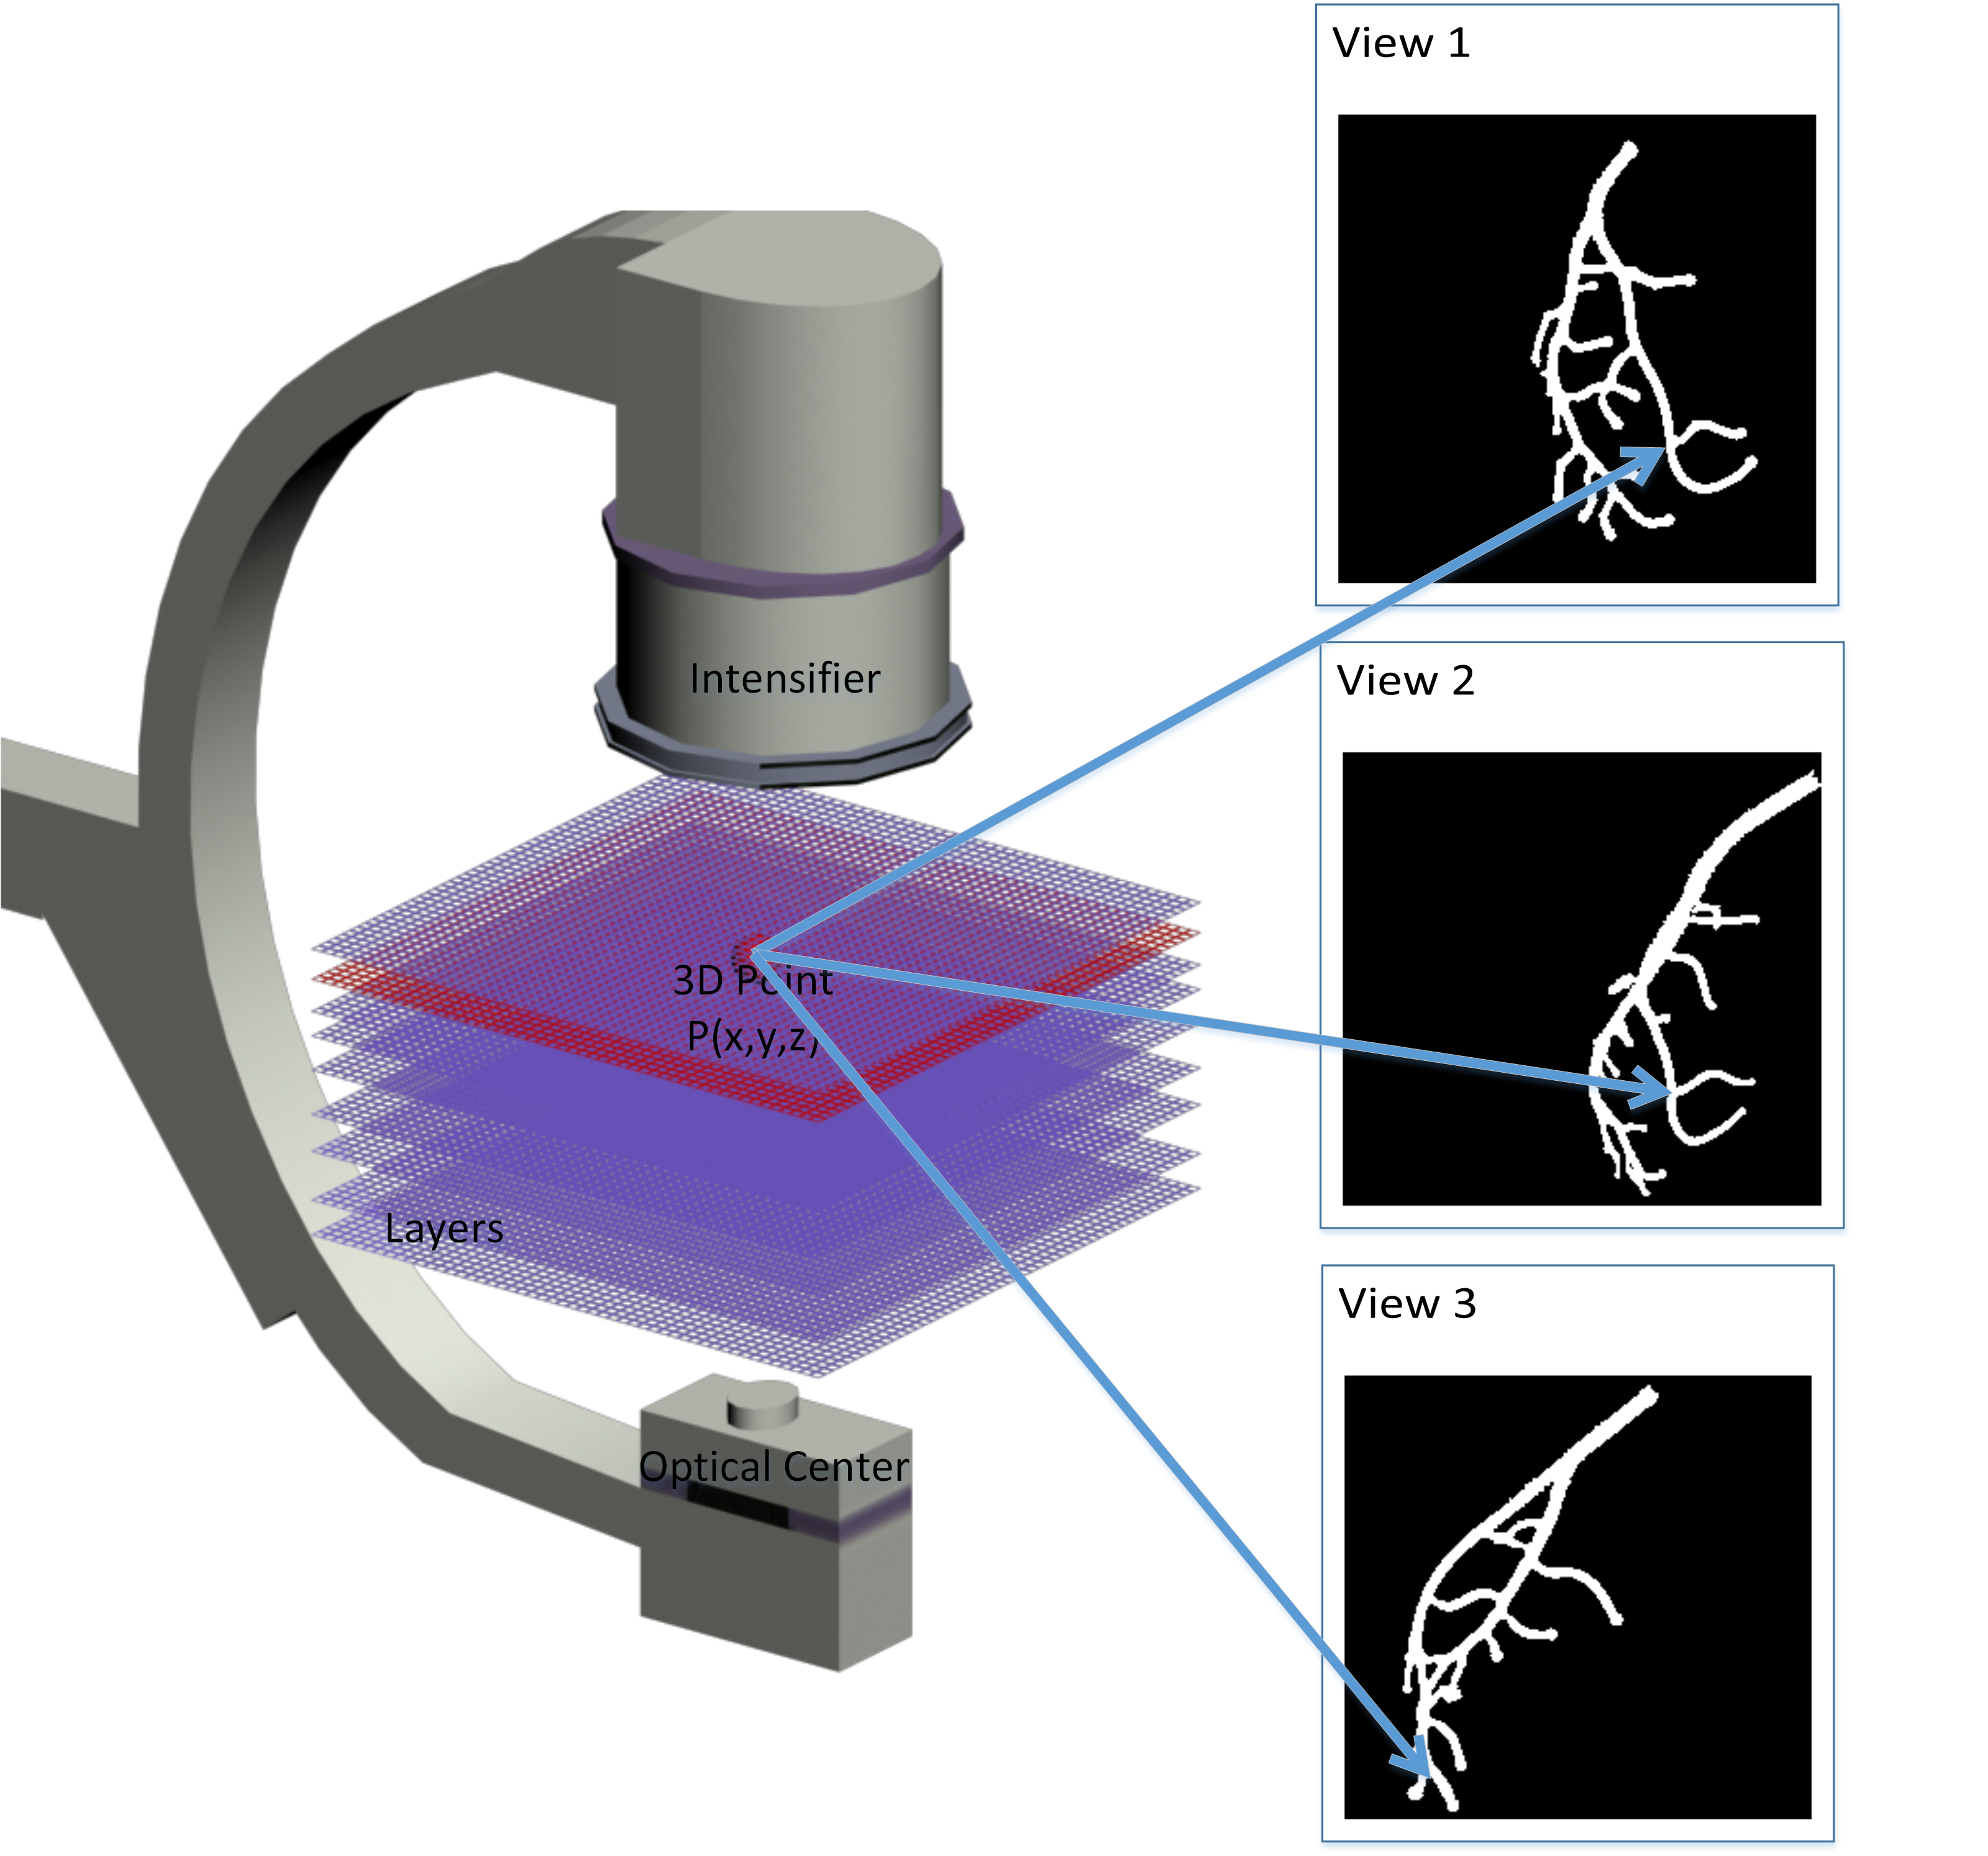
\includegraphics[width=3.0in]{c_arm_slices.png}\\
  \caption{3D Space Depth Slices}\label{fig:c_arm_slices}
\end{figure}

Each depth can be assigned with a label $l_{i}$. Meanwhile, each
skeleton point on reference view $I_{1}$ corresponds one projected
line from the source to the intensifier through all the layers.

Therefore, for a given pixel $p$ on $I_{1}$, the pair $(p,
l_{i})$ uniquely identifies a point in 3D space. So, the goal of the
3D reconstruction is to optimally assign an label $l_{i}$ to each $p$
on the centerline of the reference view $I_{1}$.  This problem can be
formulated as an energy minimization problem considering connectivity
and topological structures.The energy equation could be defined as

\begin{equation}
E(f) = \sum_{p\in P} D_{p}(f_{p}) + \lambda \sum_{p,q \in N} V_{p,q}(f_{p}, f_{q})
\end{equation}

Our goal is to find the minimum $E(f)$ and we use the belief propagation (BP)
method to achieve the solution.

In our method, we define the $V_{p,q}(f_{p}, f_{q})$ as the Euclidean
distance between point $p, q$. And we define the $D_{p}(f_{p})$ as the
\emph{color consistency} which can be described as

\begin{equation}
D_{p}(f_{p}) = \frac{1}{(n-1)} \sum_{i=2}^{n} P_{i}(x,y)
\end{equation}

where $P_{ith}(x,y)$ is the projection value of point $p$ on the
$ith$ view, which we define as

\begin{equation}
P_{ith}(x,y) =
\left\{
  \begin{array}{lll}
    W_{h}, & \hbox {$p(x,y) \in I_{ith}$} \\
    W_{l},  & \hbox {$\bigcup(p(x,y), 1) \notin I_{ith}$} \\
    W_{a}, & \hbox {else}
  \end{array}
\right.
\end{equation}

\begin{equation}
W_{a} = \frac{1}{N} \sum_{i=1}^{N} Val_{ith}(x,y)
\end{equation}

where $p(x,y)\in I_{ith}$ means that $p(x,y)$ is a valid centerline
point of $I_{ith}$, $W_{h}$ and $W_{l}$ are two constants that
control the very high and very low of the value. For a grey scale
image, $\bigcup(p(x,y), 1)$ is the 8 neighbors of the point
$p(x,y)$.  If $p(x,y)$ can not be found right in the $I_{ith}$, we
will compute its 8 neighbors and obtain the average value as the
value of point $p(x,y)$. And if none of its neighbors is valid, it
could be assigned with $ W_{l}$.

Our algorithm includes two main steps, message propagation and energy
minimization computation. In message propagation, the color value of
point $p(x,y) \in I_{1}$ is updated as

\begin{equation}
V_{p} = V_{p} + \alpha minD+ (1-\alpha)V_{p_{minD}})
\end{equation}

where $\alpha$ is a constant controlling the weight its neighbors'
\emph{color consistency} and \emph{dist consistency}. $minD$ stands for the minimum
distance from $p(x,y)$ to its neighbors. $V_{p_{minD}}$ stands for the
value of the minimum distance point.

In our energy minimization, different from typical BP, the current energy of the $ith$
depth($l_{i}$) is defined as

\begin{equation}
e_{i}(p_{i}) = min[\gamma D(p_{i}, q) + (1-\gamma)V(q) + e_{i-1}(q)];
\end{equation}

in which $q$ stands for the projected sample depths of
$\bigcup^\circ(p_{i}, 1)$ which is the neighbours of $p_{i}$ without including $p_{i}$
itself.

At last, we compute the minimum sum of all the grouped vessel skeletons' cost,
and obtain the optimal solution for the whole vessel skeleton tree.

After the reconstruction of the 3D skeletons of the coronary arteries,
using the diameters we extracted, we obtain the final result as shown in
Figure \ref{fig:final_result}.




\begin{figure}
  \centering
  % Requires \usepackage{graphicx}
  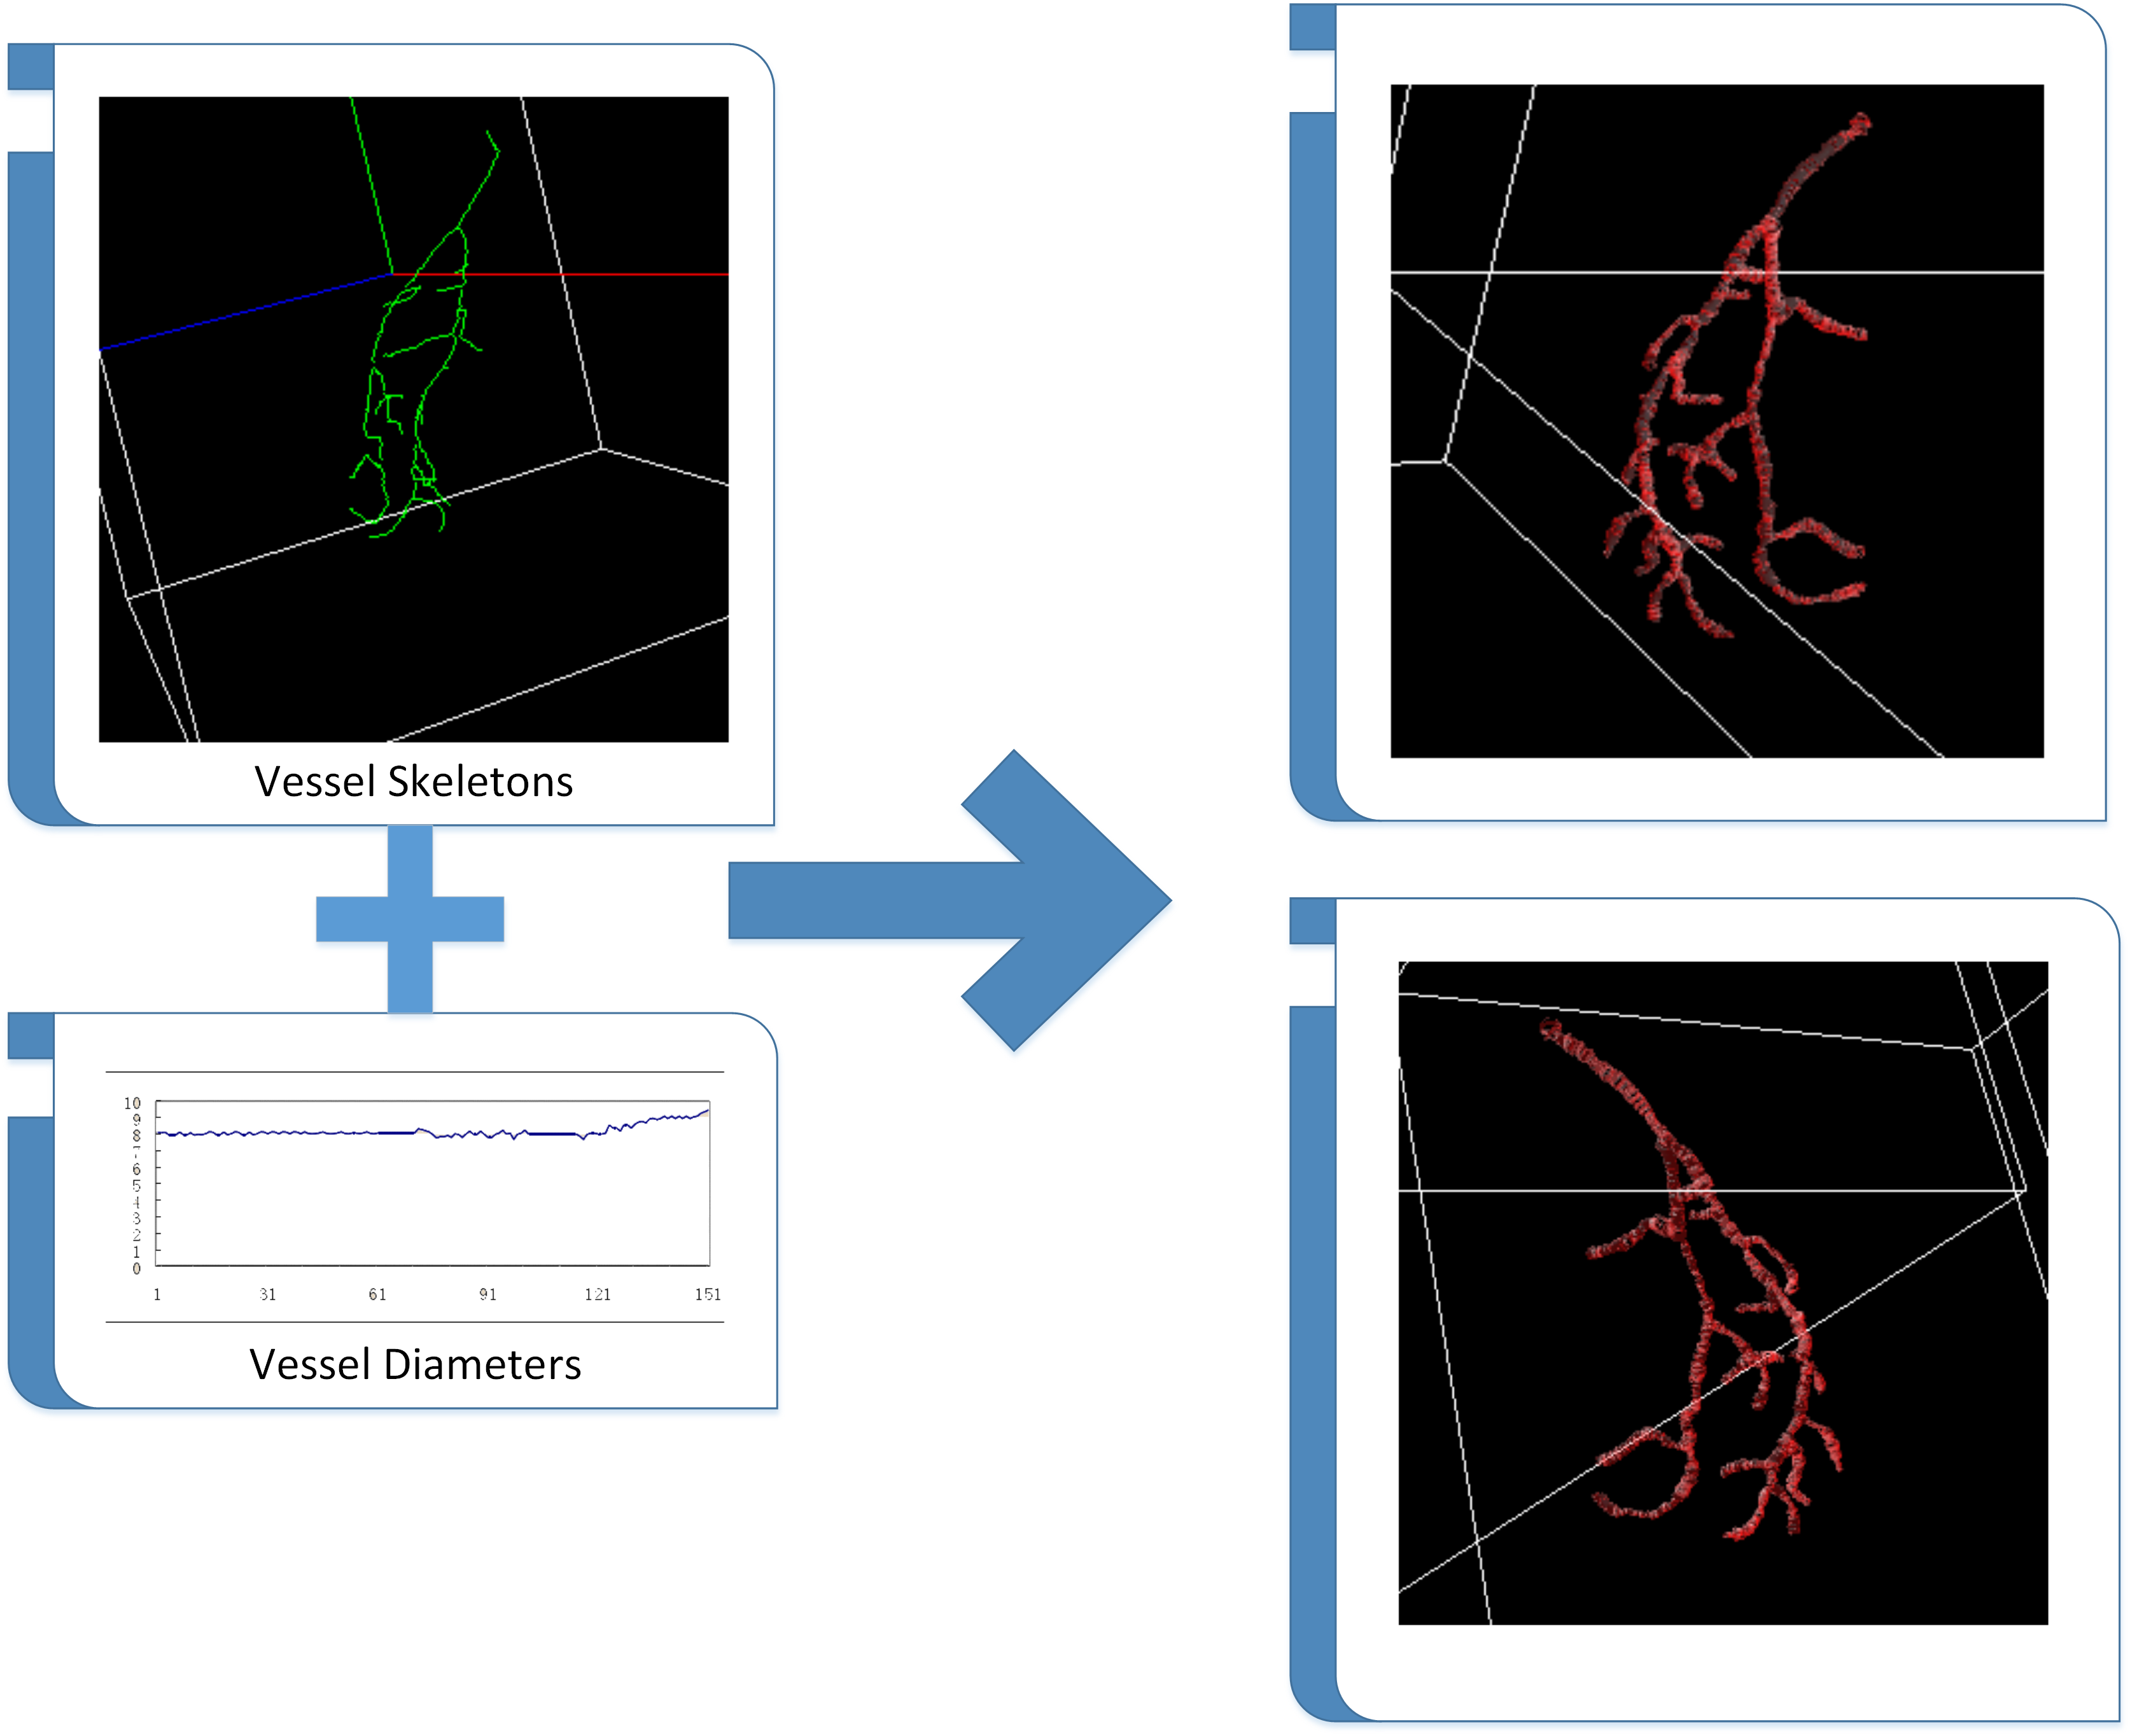
\includegraphics[width=3.0in]{final_result.png}
  \caption{The Skeleton with Diameters}
  \label{fig:final_result}
\end{figure}
